\chapter[Aplicaciones]{Aplicaciones}

A continuaci\'on se exponen los resultados de utilizar el paquete de R \textit{GPDPQuantReg}, mismo que, como se detalló en el cap\'itulo anterior, implementa el modelo \textit{GPDP} para la regresi\'on sobre cuantiles.

En primer lugar se presenta el ajuste del modelo en datos simulados, con el fin de comparar los resultados con los valores conocidos de antemano. Posteriormente se presenta para dos conjuntos de datos reales, con la intenci\'on de obtener conclusiones en aplicaciones pr\'acticas, mediante el uso del modelo central de esta tesis.

\section{Simulaci\'on}

Los datos de esta secci\'on se obtuvieron de la siguiente manera. Sea $y \in \mathbb{R}$ el valor de la variable de respuesta, $x \in \mathbb{R}$ su respectiva covariable, $g: \mathbb{R} \rightarrow \mathbb{R}$ la funci\'on denominada \textit{originaria} y $E \in \mathbb{R}$ un error aleatorio, se simul\'o:
\begin{equation*}
    y = g(x) + E.
\end{equation*}
Las diferencias entre las subsecciones siguientes radican en variaciones del valor de $g$ y la distribuci\'on de $E$.

Dada esta construcci\'on, la funci\'on real del cuantil p-\textit{\'esimo} de $y|x$ se puede obtener como
\begin{equation*}
    q_p(y|x) = g(x) + q_p(E),
\end{equation*}
la cual se estimar\'a para diversos valores de $p$.

En todos los casos se ajust\'o el modelo para los cuantiles $0.5$\textit{-\'esimo}, por ser la mediana y una medida de tendencia central; el $0.95$\textit{-\'esimo}, dado que es un valor extremo, y el $0.25$\textit{-\'esimo}, debido a que es el primer cuartil, y no es ni medida de tendencia central, pero tampoco un valor extremo.

Por otro lado, para todos los casos se simularon 40 datos sin reemplazo, dentro del intervalo $(-15,15)$, con un refinamiento de 3 decimales.

\subsection{Funci\'on simple, error simple}

Para obtener este conjunto de datos se utiliz\'o una funci\'on originaria $g$ considerada simple: la cuadr\'atica
\begin{equation*}
    g(x) = \frac{1}{40}x^2 - \frac{1}{20}x - 2.
\end{equation*}
Por otro lado, el error $E \sim \mathcal{N}(0,1)$ tambi\'en fue sencillo, debido a que fue sim\'etrico y no acotado. Los datos simulados se pueden observar en la figura \ref{sample_sgse}.

Posteriormente se ajust\'o el modelo y se realiz\'o predicci\'on sobre un refinamiento del intervalo simulado de $x$, obteniendo buenos resultados (figura \ref{fitted_sgse}), ya que las funciones reales de los diversos cuantiles cayeron en su totalidad dentro del intervalo de probabilidad al 90\%, estimado por el modelo. Adem\'as, las medianas de la distribuciones posteriores siguieron un comportamiento similar a las originales.

Por otro lado, como se detall\'o en el cap\'itulo anterior, con el uso del paquete \textit{GPDPQuantReg} tambi\'en es posible obtener varios diagn\'osticos de las cadenas de markov. Por ejemplo, se presentan los del cu\'antil $0.5$-\textit{\'esimo} en la figura \ref{diag_sgse}, mismos que reflejan un buen desempeño del algoritmo.

\begin{figure}[H]
	\centering
	\caption{Datos simulados y cuantiles de referencia, para funci\'on simple y error simple}
	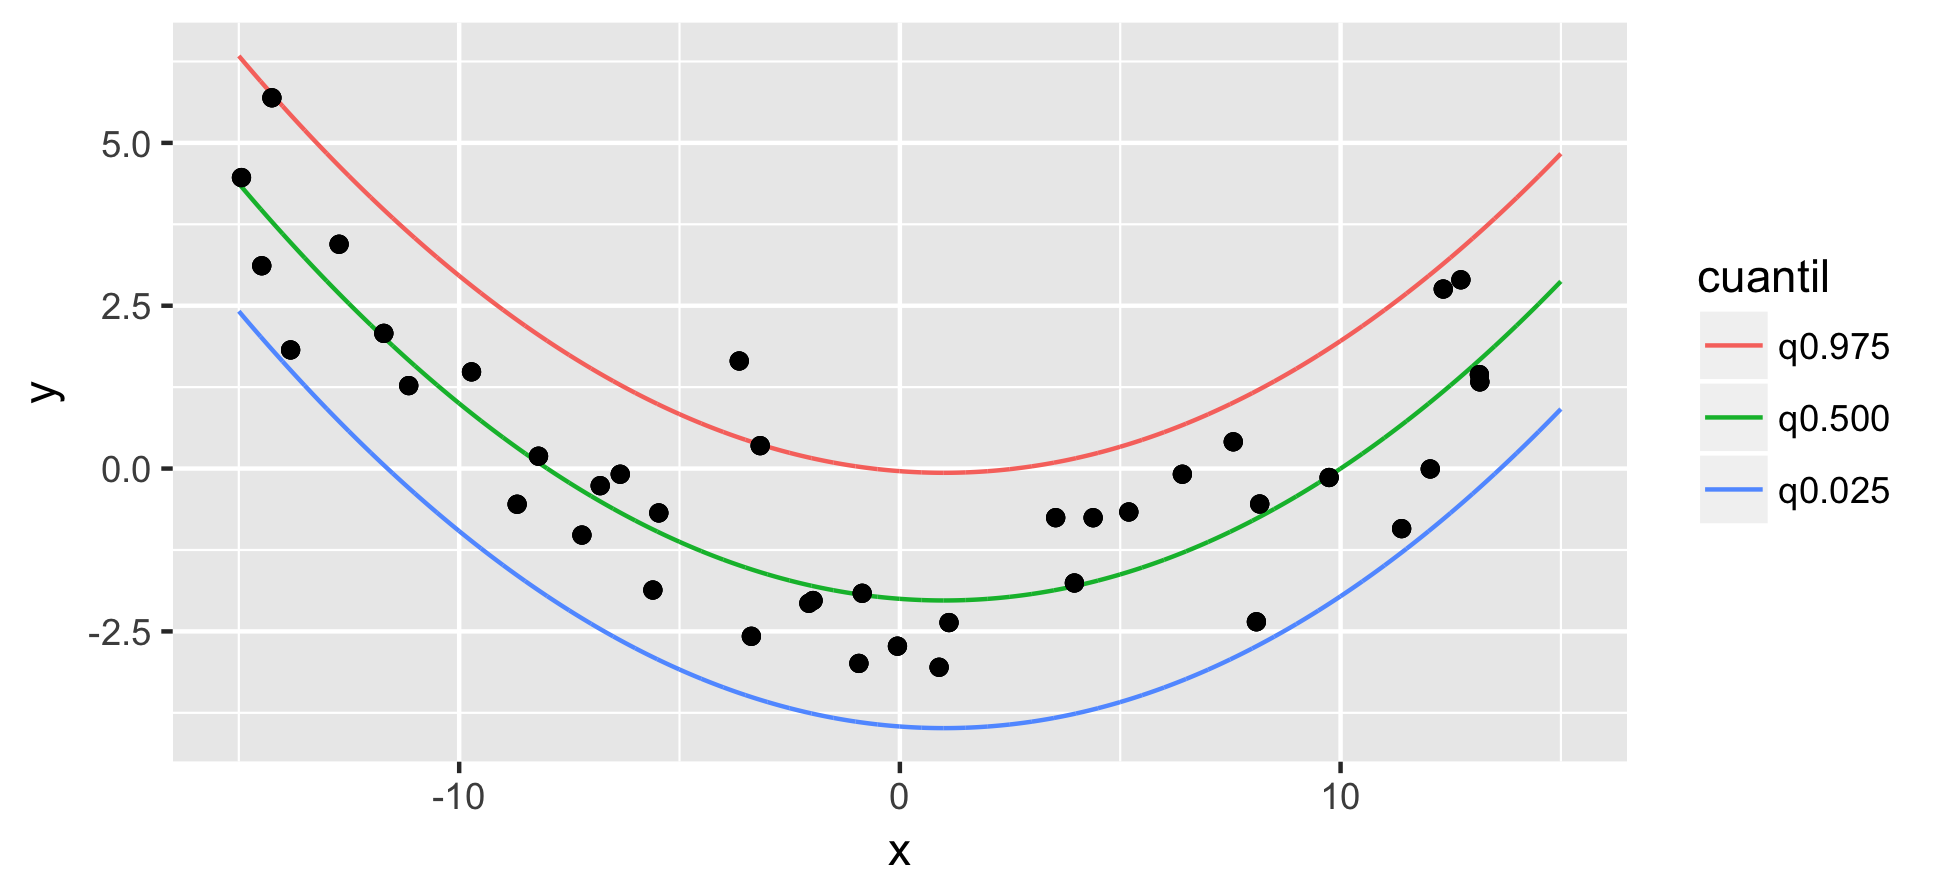
\includegraphics[width=0.60\textwidth]{Figures/Simulation/simple_g_simple_error/sample.png}
	\label{sample_sgse}
\end{figure}

\begin{figure}[H]
	\centering
	\caption{Ajuste del modelo \textit{GPDP}, para funci\'on simple y error simple}
	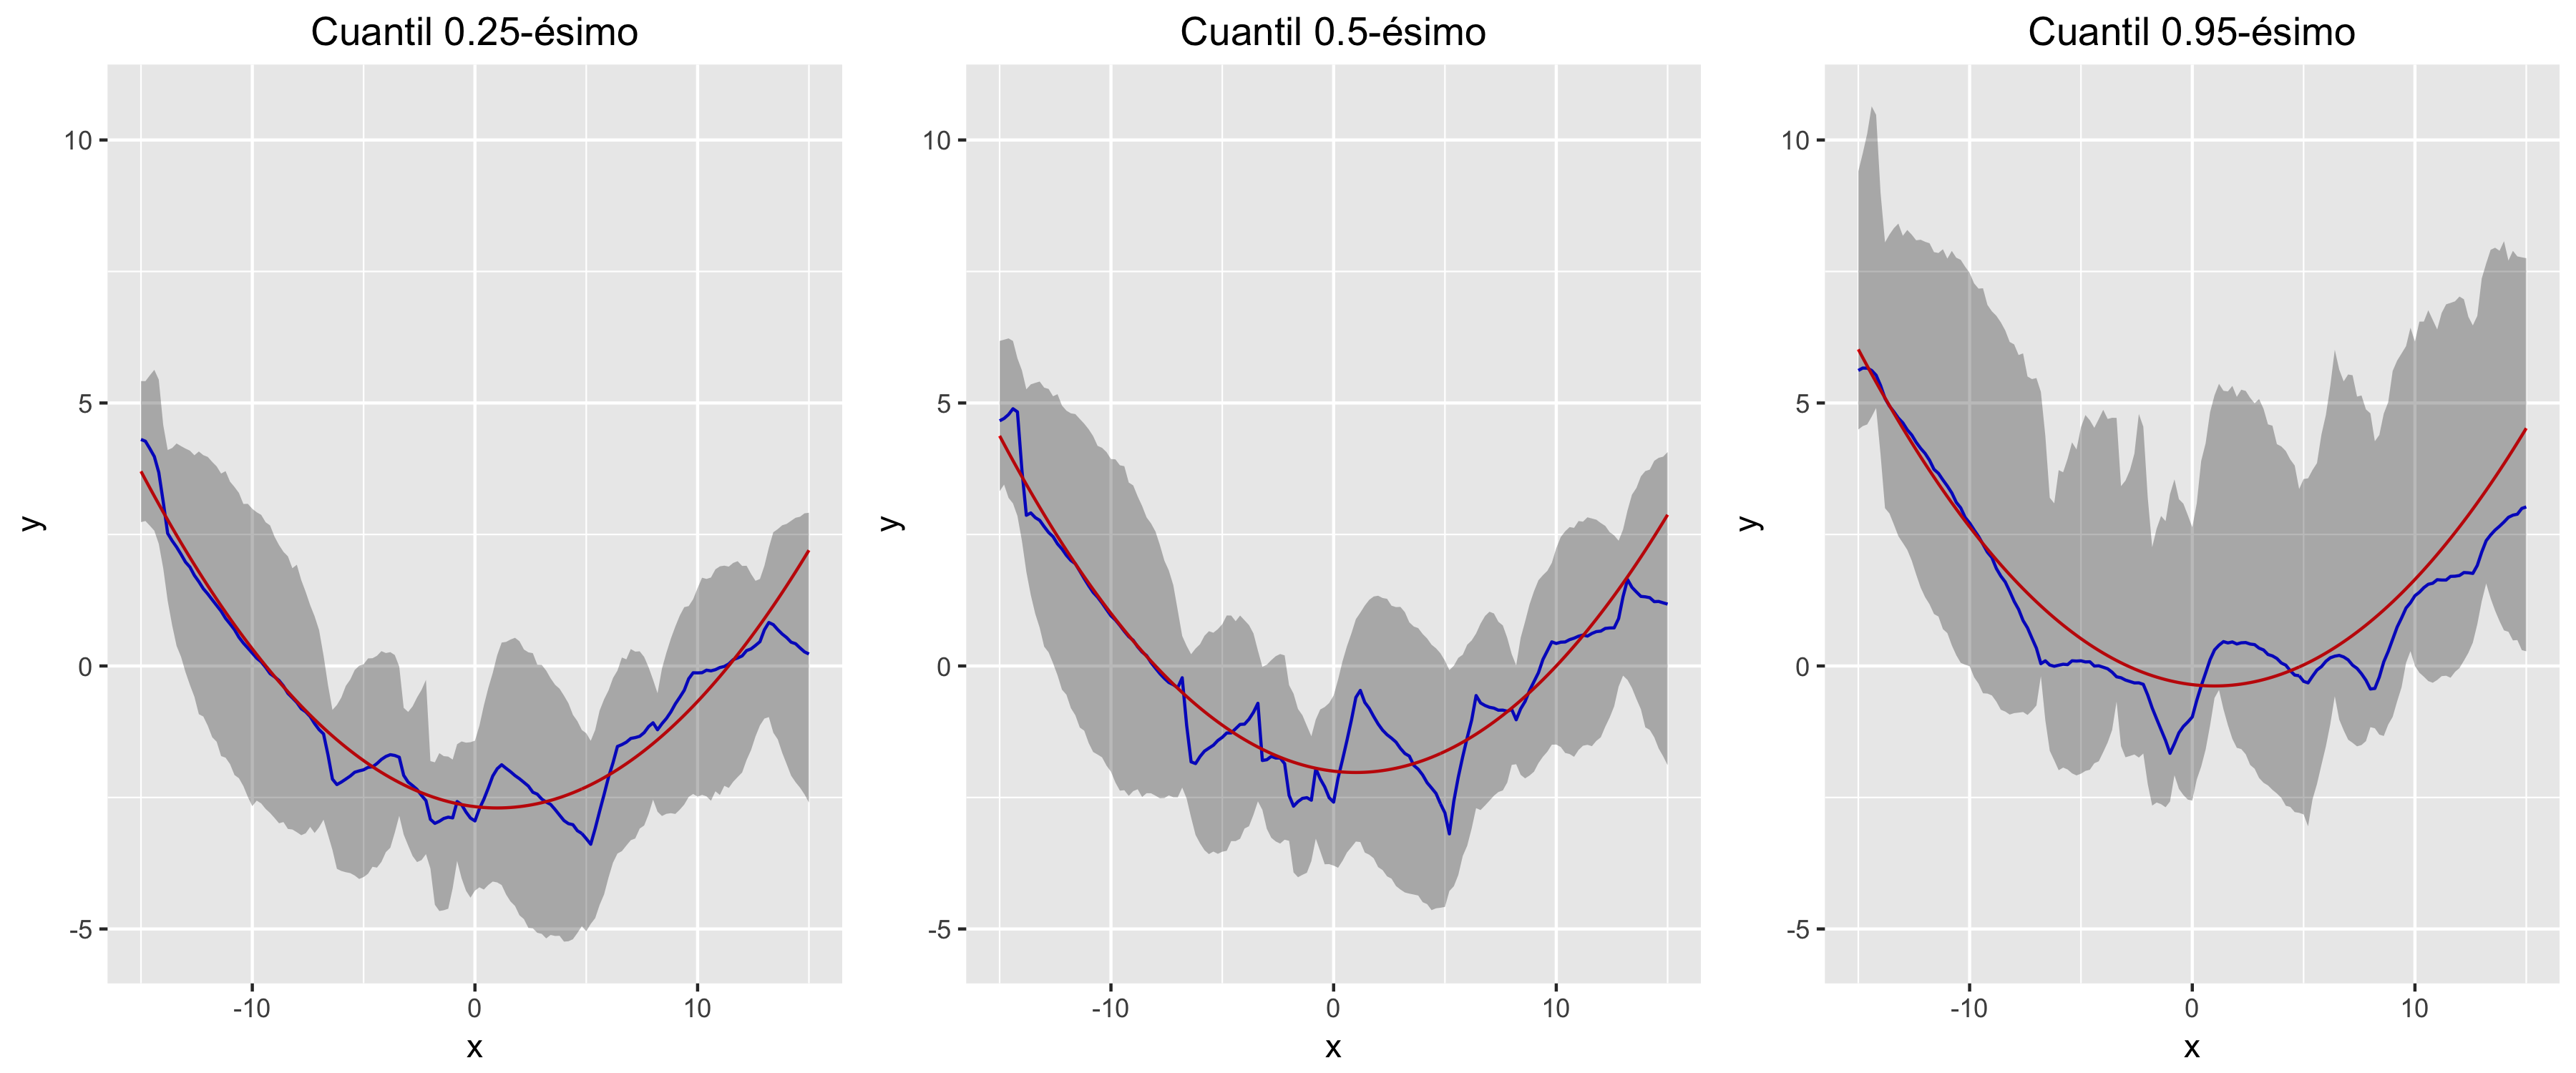
\includegraphics[width=\textwidth]{Figures/Simulation/simple_g_simple_error/fitted_models.png}
	\captionsetup{singlelinecheck=off,font=footnotesize}
    \caption*{La l\'inea roja representa el valor real de cada cuantil, la l\'inea azul representa la mediana de la distribuci\'on posterior predictiva y el \'area gris su intervalo de probabilidad al 90\%.}
	\label{fitted_sgse}
\end{figure}

\begin{figure}[H]
	\centering
	\caption{Diagn\'osticos de las cadenas de markov del cu\'antil $0.5$-\textit{\'esimo}, para funci\'on simple y error simple}
	\subfloat[Ergodicidad]{
	    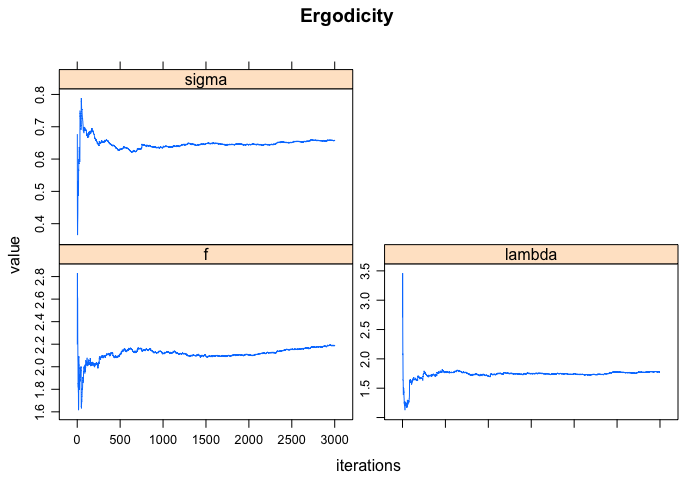
\includegraphics[width=0.45\textwidth]{Figures/Simulation/simple_g_simple_error/ergodicity.png}
	}
	\subfloat[Autocorrelaci\'on]{
	    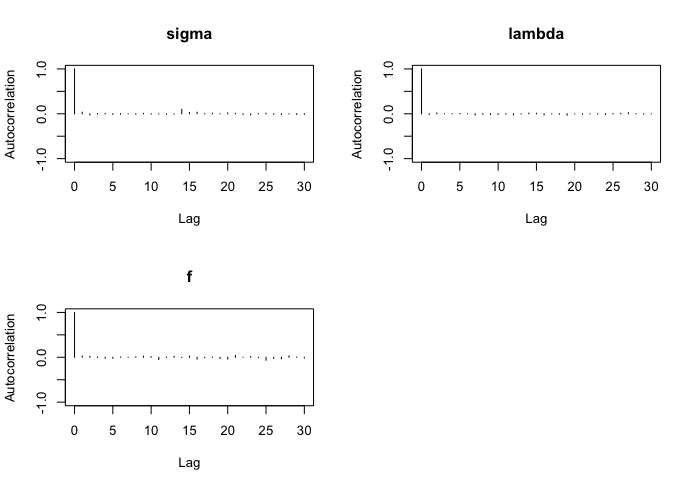
\includegraphics[width=0.45\textwidth]{Figures/Simulation/simple_g_simple_error/autocorrelation.png}
	}\\
	\subfloat[Correlaci\'on cruzada]{
	    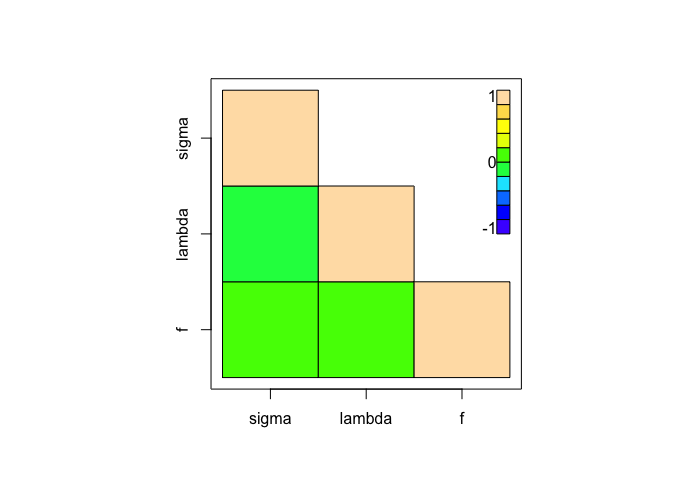
\includegraphics[width=0.45\textwidth]{Figures/Simulation/simple_g_simple_error/crosscorrelation.png}
	}
	\subfloat[Traza]{
	    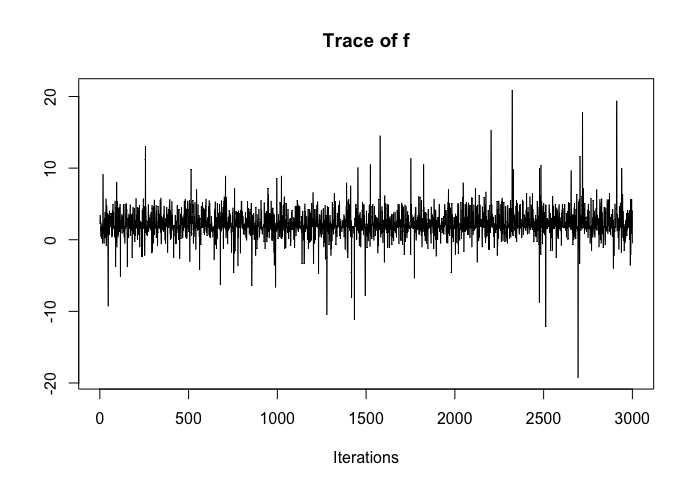
\includegraphics[width=0.45\textwidth]{Figures/Simulation/simple_g_simple_error/trace.png}
	}
	\label{diag_sgse}
\end{figure}

\subsection{Funci\'on compleja, error simple}

En este caso, se mantuvo que $E \sim \mathcal{N}(1,0)$, pero la funci\'on $g$ usada fue m\'as compleja:
\begin{equation*}
    g(x) = \frac{1}{2} x \cos(x) - \exp\left(\frac{1}{10}x\right).
\end{equation*}

Los datos simulados se pueden observar en la figura \ref{sample_cgse}, los cuales al ajustar el modelo, mostraron de nuevo buenos resultados (figura \ref{fitted_cgse}), al aparecer la funci\'on original adentro del intervalo de probabilidad al 90\% en pr\'acticamente todos los valores de $x$ en los que se realiz\'o predicci\'on, a excepci\'on de la \'ultima zona, n la que no hubo datos de entrenamiento.

\begin{figure}[H]
	\centering
	\caption{Datos simulados y cuantiles de referencia, para funci\'on compleja y error simple}
	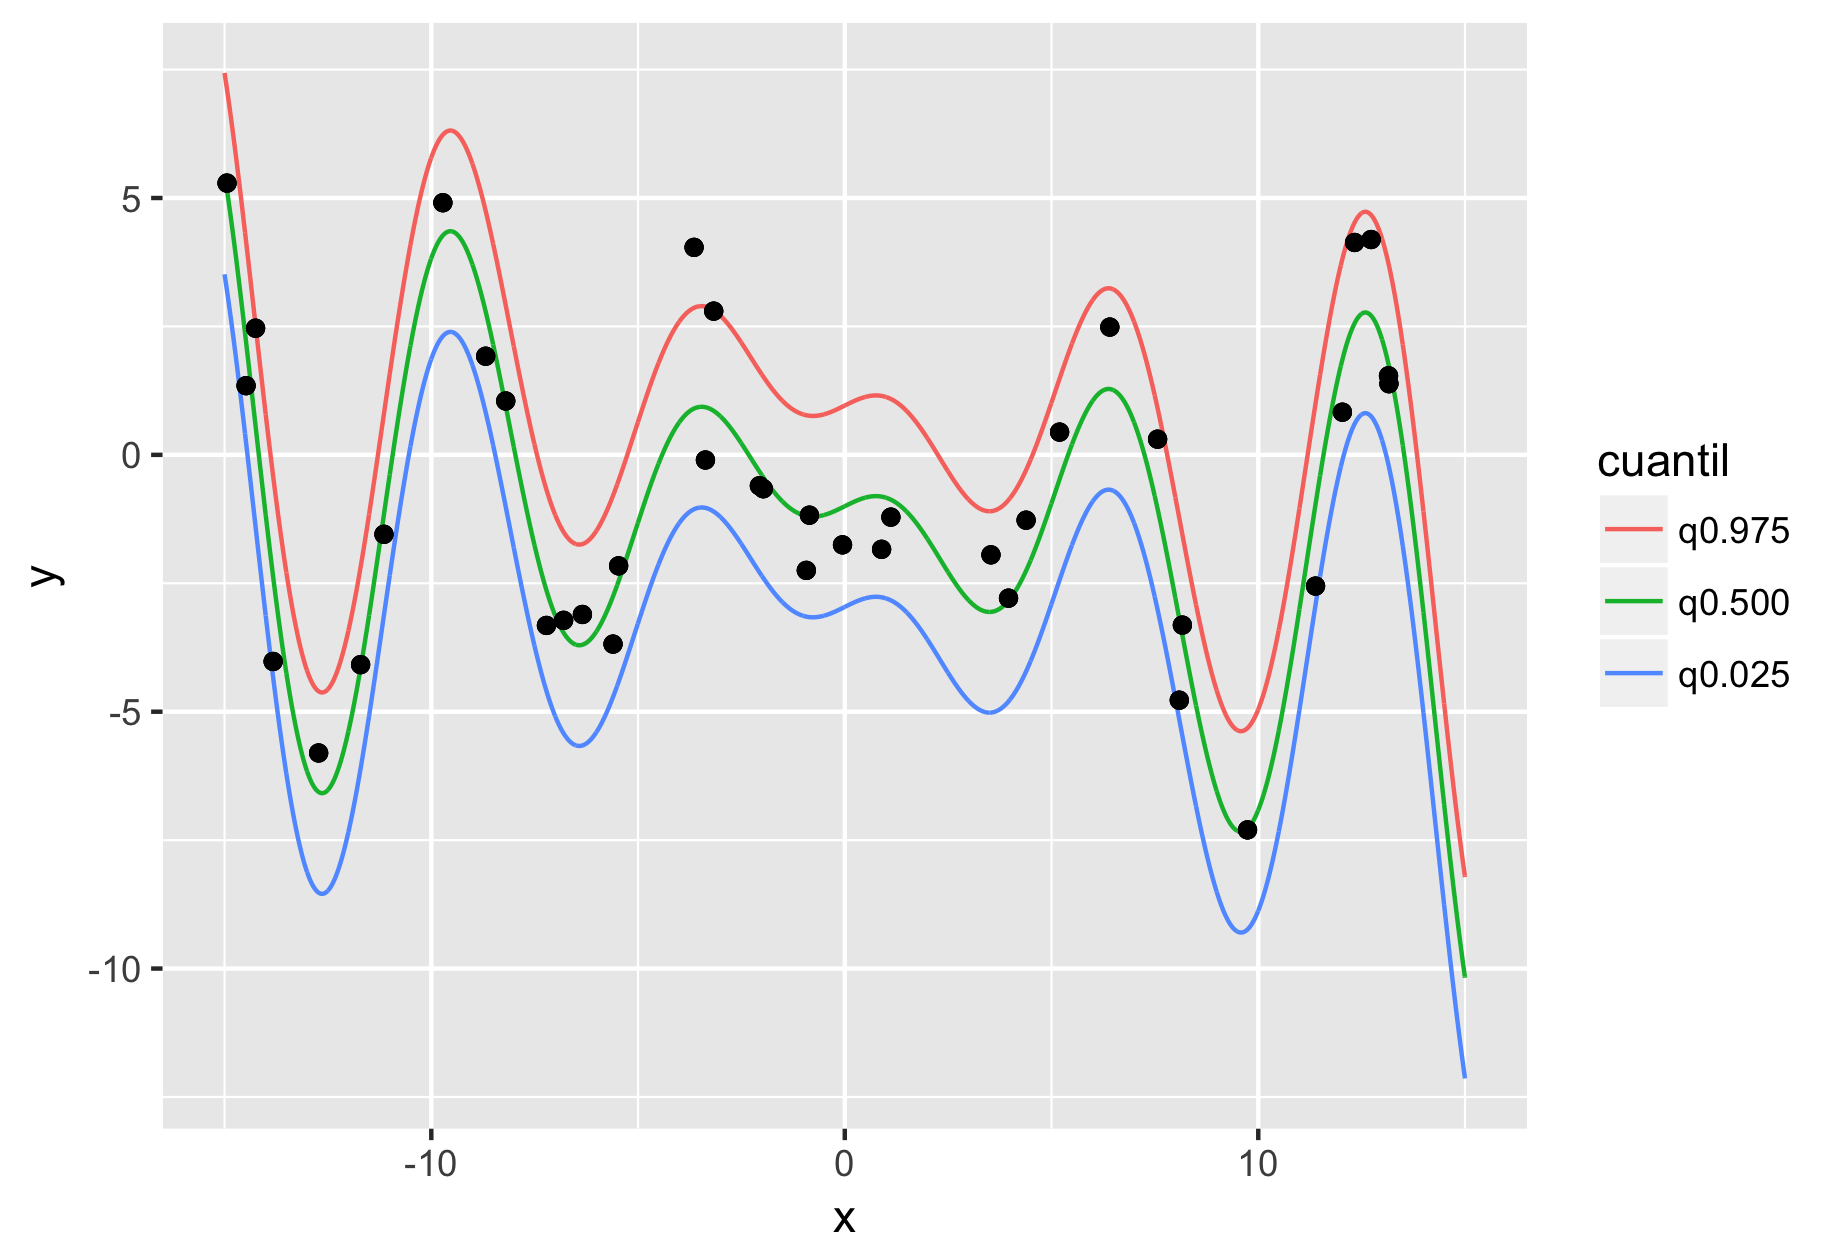
\includegraphics[width=0.60\textwidth]{Figures/Simulation/complex_g_simple_error/sample.png}
	\label{sample_cgse}
\end{figure}

\begin{figure}[H]
	\centering
	\caption{Ajuste del modelo \textit{GPDP}, para funci\'on compleja y error simple}
	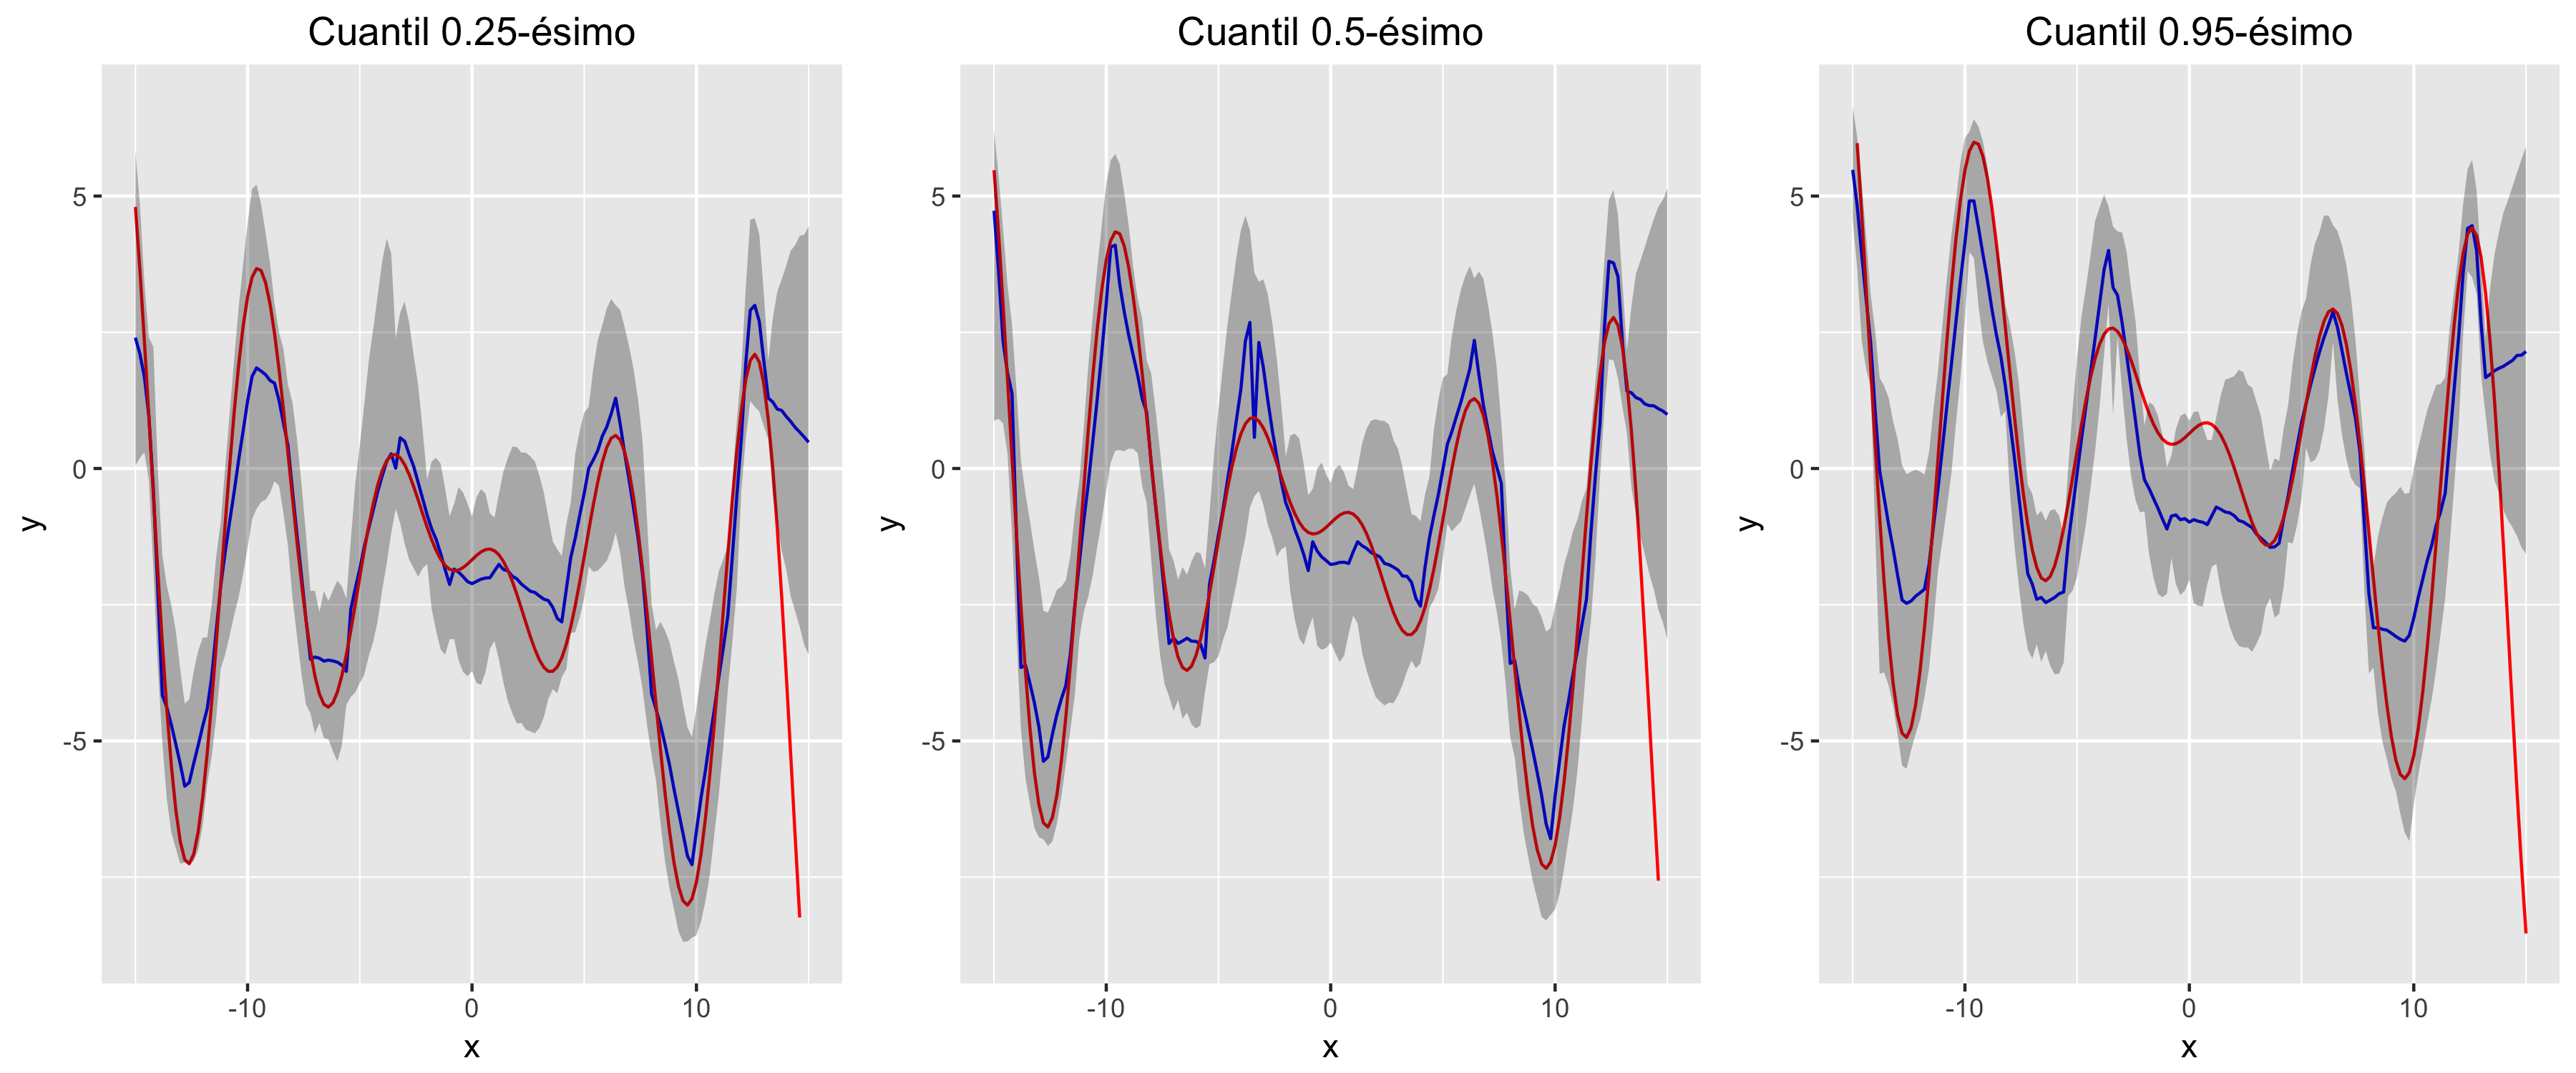
\includegraphics[width=\textwidth]{Figures/Simulation/complex_g_simple_error/fitted_models.png}
	\captionsetup{singlelinecheck=off, font=footnotesize}
    \caption*{La l\'inea roja representa el valor real de cada cuantil, la l\'inea azul representa la mediana de la distribuci\'on posterior predictiva y el \'area gris su intervalo de probabilidad al 90\%.}
	\label{fitted_cgse}
\end{figure}

\subsection{Funci\'on simple, error complejo}

En este caso, se uso una funci\'on lineal $g$:
\begin{equation*}
    g(x) = \frac{1}{2} x.
\end{equation*}
La complejidad se introdujo en $E \sim \textit{Gamma}(\alpha = 2,\beta = 1)$, debido a que el error no fue sim\'etrico y fue acotado por la izquierda. 

El conjunto de datos usado para este modelo aparece en la figura \ref{sample_sgce}, y a pesar de la complejidad del error, se obtuvieron buenos resultados (figura \ref{fitted_sgce}), debido a que nuevamente las funciones reales de los diversos cuantiles cayeron en su totalidad dentro del intervalo de probabilidad al 90\%, estimado por el modelo.

Un detalle notable es que, al igual que el caso de funci\'on simple y error simple, la estimaci\'on de la funci\'on del cuantil 0.95\textit{-\'esimo} muestra una varianza m\'as grande que los otros dos cuantiles. Esto debido a que en valores extremos el modelo refleja mayor incertidumbre de lo que en realidad podr\'ia estar ocurriendo.

\begin{figure}[H]
	\centering
	\caption{Datos simulados y cuantiles de referencia, para funci\'on simple y error complejo}
	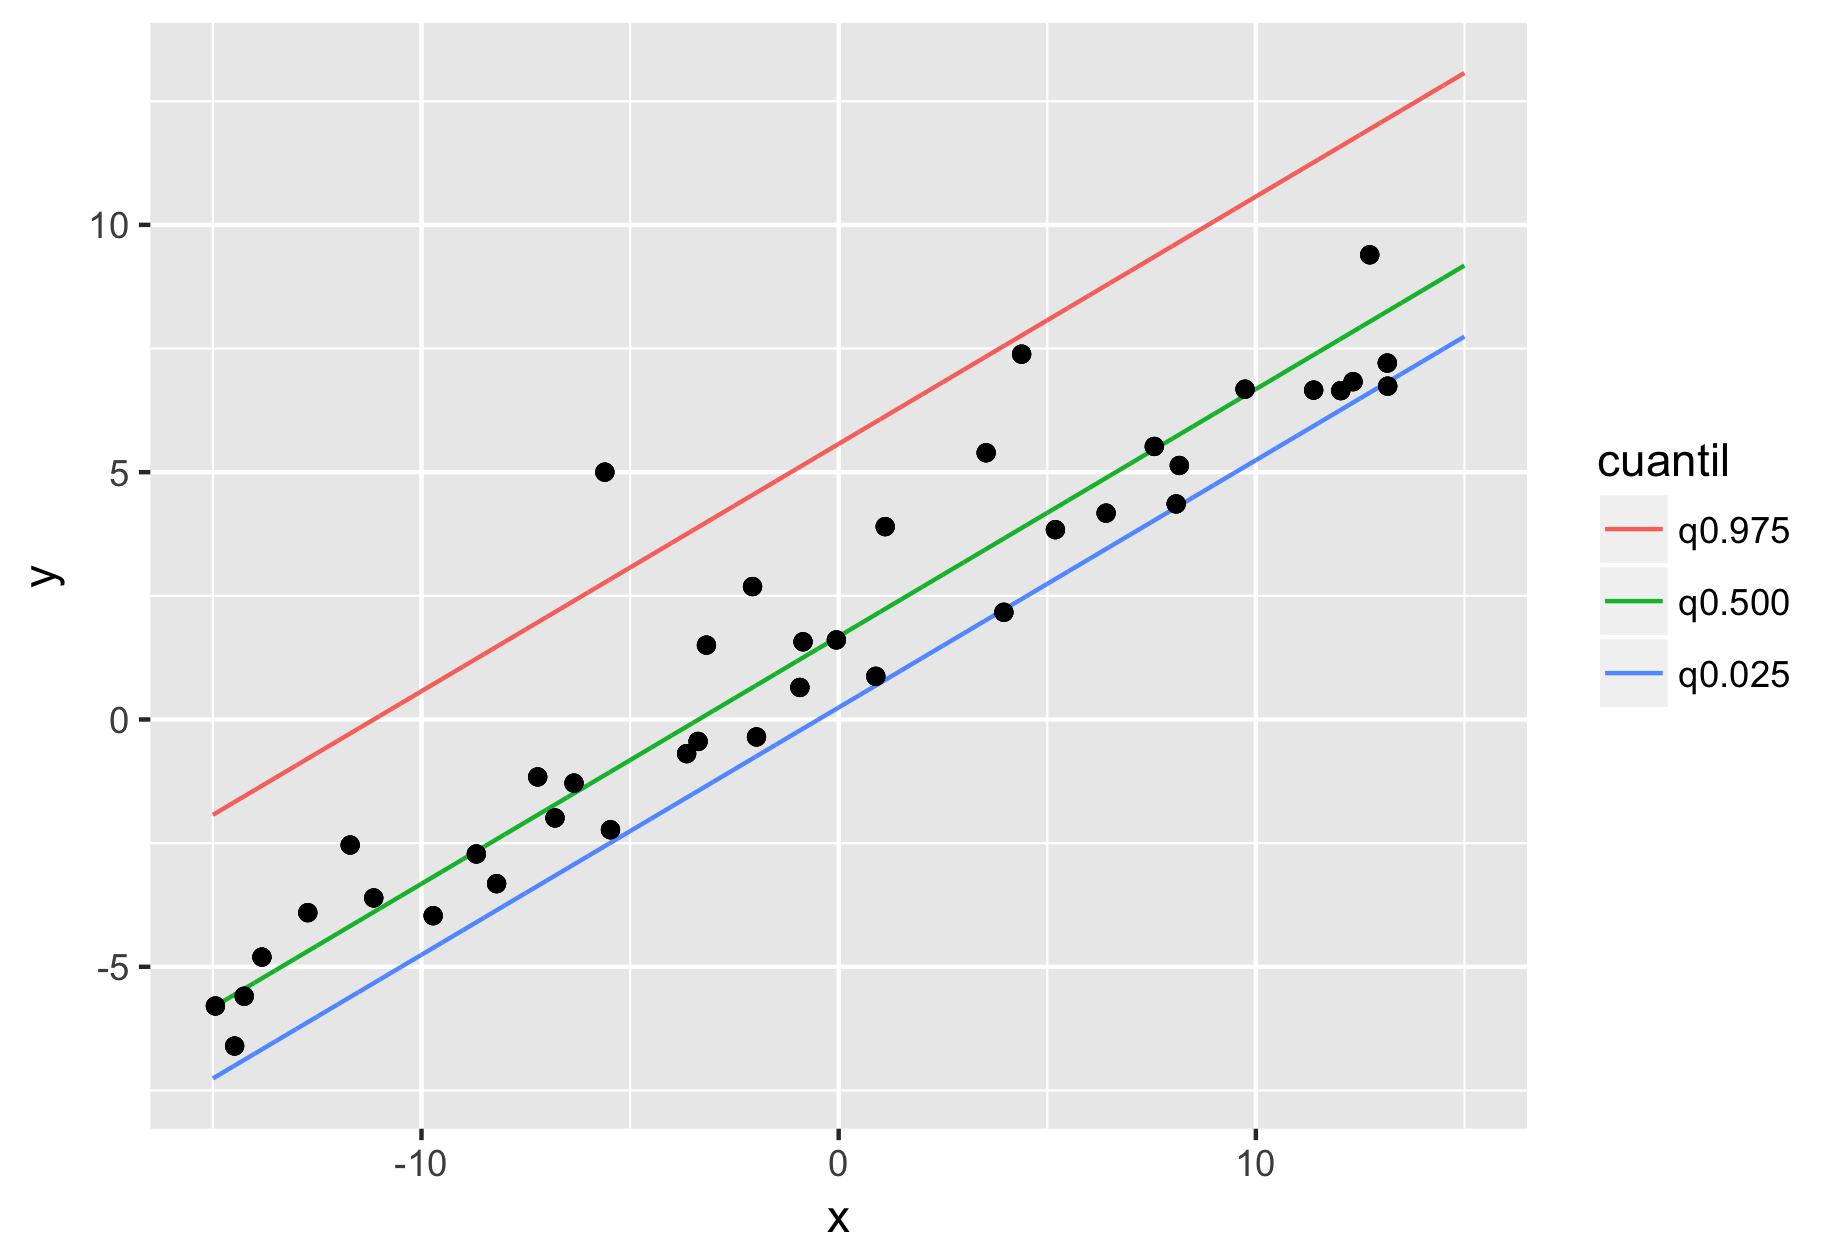
\includegraphics[width=0.60\textwidth]{Figures/Simulation/simple_g_complex_error/sample.png}
	\label{sample_sgce}
\end{figure}

\begin{figure}[H]
	\centering
	\caption{Ajuste del modelo \textit{GPDP}, para funci\'on simple y error complejo}
	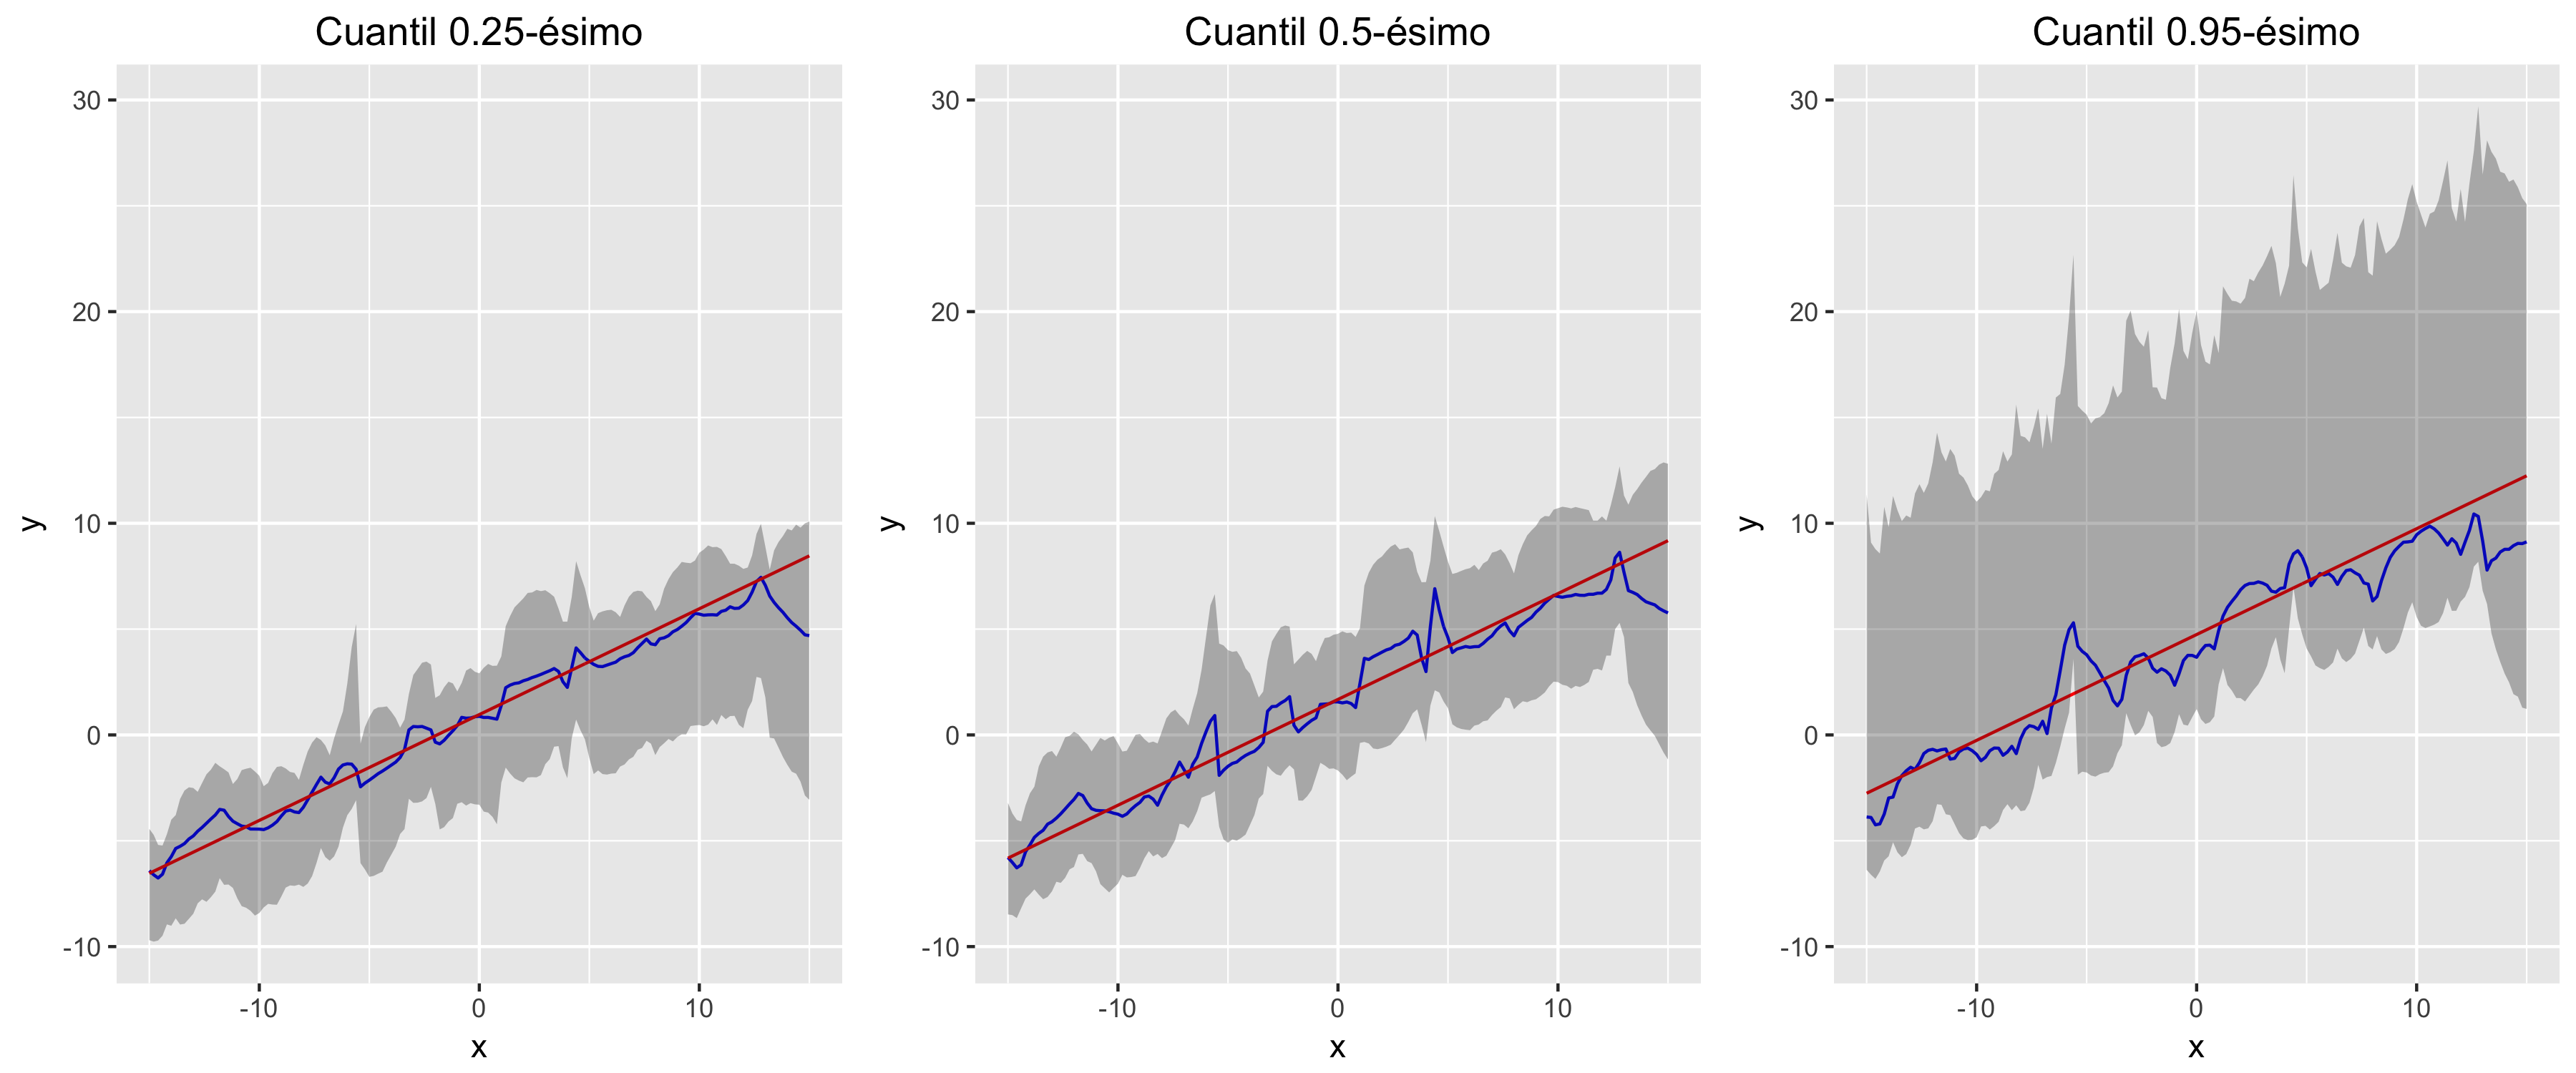
\includegraphics[width=\textwidth]{Figures/Simulation/simple_g_complex_error/fitted_models.png}
	\captionsetup{singlelinecheck=off,font=footnotesize}
    \caption*{La l\'inea roja representa el valor real de cada cuantil, la l\'inea azul representa la mediana de la distribuci\'on posterior predictiva y el \'area gris su intervalo de probabilidad al 90\%.}
	\label{fitted_sgce}
\end{figure}

\subsection{Funci\'on compleja, error complejo}

En este modelo se usaron datos (figura \ref{sample_cgce}) provenientes tanto de un error complejo, $E \sim \textit{Gamma}(\alpha = 2,\beta = 1)$, como de una funci\'on $g$ compleja:
\begin{equation*}
    g(x) = \frac{1}{2} x \cos(x) - \exp\left(\frac{1}{10}x\right).
\end{equation*}

Despu\'es del ajuste (figura \ref{fitted_cgce}), el balance fue positivo, debido a que las funciones reales de los diversos cuantiles cayeron en su totalidad dentro del intervalo de probabilidad al 90\%, del estimado por el modelo, a excepci\'
on de la zona de la que no se tuvieron datos, como en el caso de funci\'on compleja y error simple. Pero a diferencia de ese modelo, el error complejo produce una mayor incertidumbre, particularmente notoria en el caso del cuantil 0.95\textit{-\'esimo}.

\begin{figure}[H]
	\centering
	\caption{Datos simulados y cuantiles de referencia, para funci\'on compleja y error complejo}
	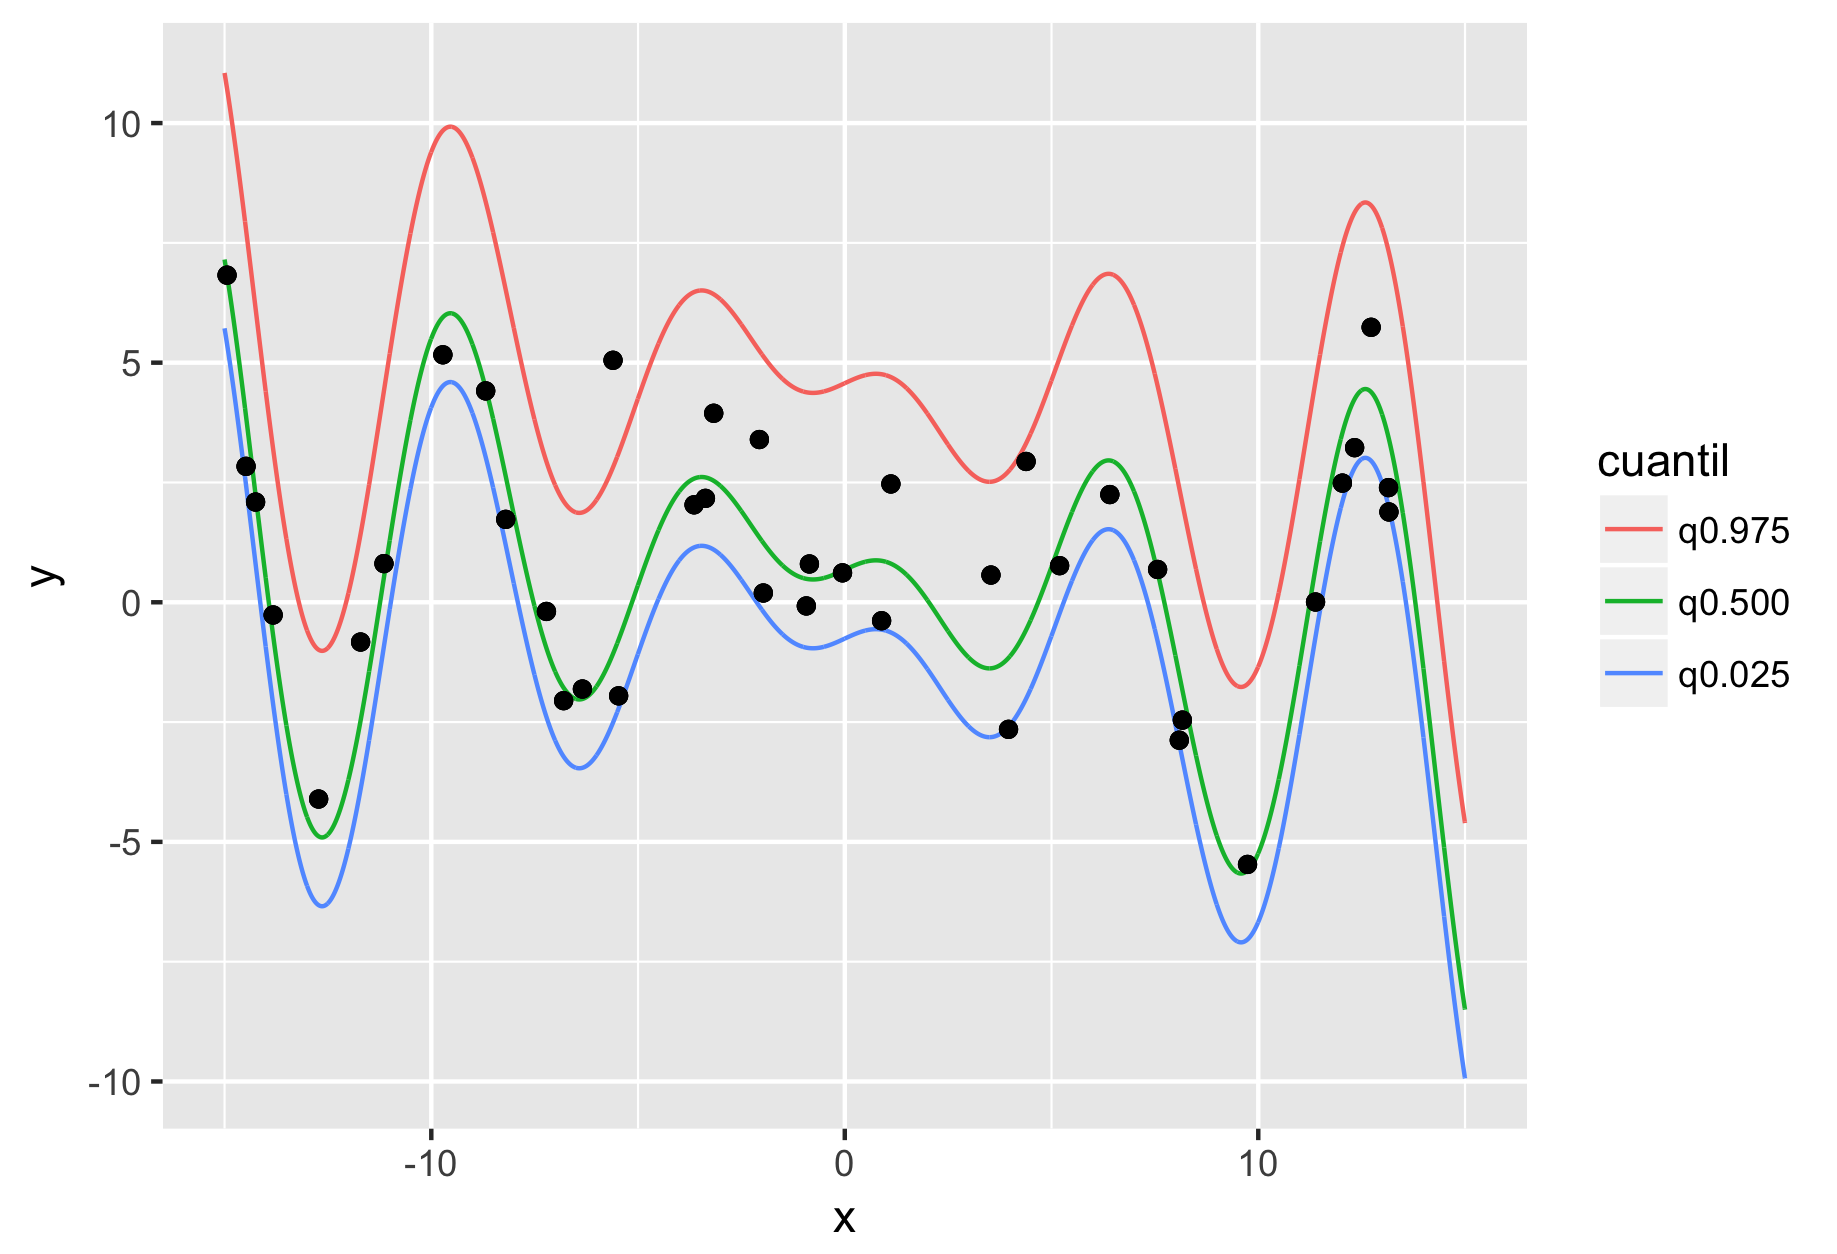
\includegraphics[width=0.60\textwidth]{Figures/Simulation/complex_g_complex_error/sample.png}
	\label{sample_cgce}
\end{figure}

\begin{figure}[H]
	\centering
	\caption{Ajuste del modelo \textit{GPDP}, para funci\'on compleja y error complejo}
	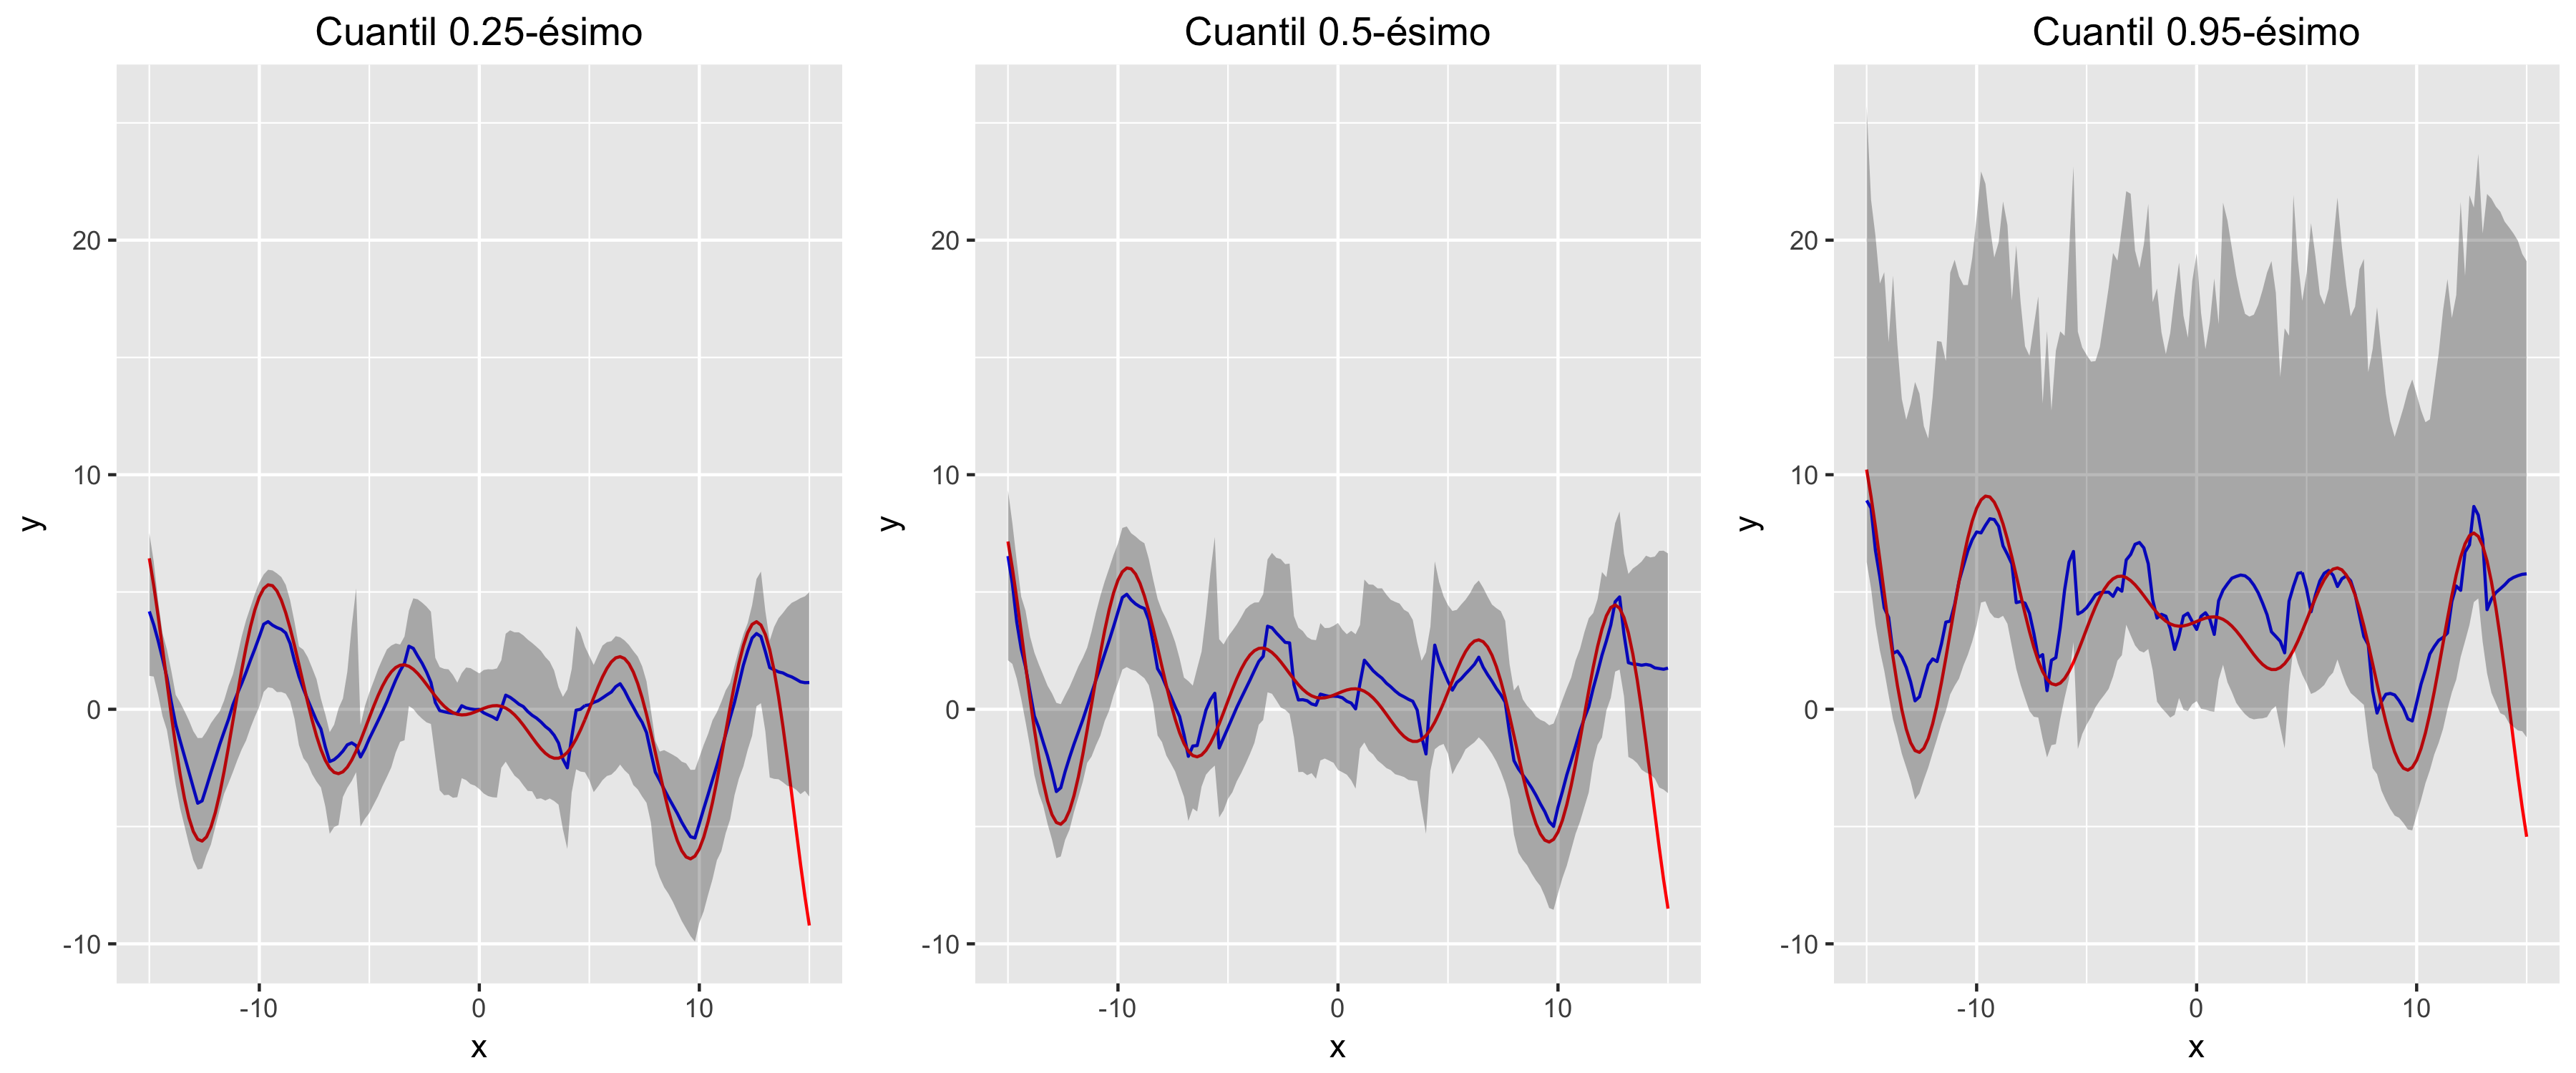
\includegraphics[width=\textwidth]{Figures/Simulation/complex_g_complex_error/fitted_models.png}
	\captionsetup{singlelinecheck=off,font=footnotesize}
    \caption*{La l\'inea roja representa el valor real de cada cuantil, la l\'inea azul representa la mediana de la distribuci\'on posterior predictiva y el \'area gris su intervalo de probabilidad al 90\%.}
	\label{fitted_cgce}
\end{figure}

\section{Sector salud}


\section{Tipo de cambio}

\newpage